\chapter{Test13}


\begin{figure}
\begin{center}
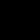
\includegraphics[width=\maxwidth]{x}
\caption[Dies ist die Beschriftung zu X]{Dies ist die Beschriftung zu X}
\label{seq:refIllustration0}

\end{center}
\end{figure}
Dies ist ein Text! In Abbildung \ref{seq:refIllustration0} zu sehen ist.


Das ist \figurename~\ref{seq:refIllustration0}.

\begin{longtable}[c]{|m{3.199cm}|m{3.199cm}|m{3.199cm}|m{3.199cm}|m{3.199cm}|}

\endhead
\hline
\centering \bfseries Haus&
\centering \bfseries Stra�e&
\centering \bfseries plz&
\centering \bfseries Ort&
\centering\arraybslash \bfseries xxx\\\hline
&
&
&
&
\\\hline
&
&
&
&
\\\hline
&
&
&
&
\\\hline
\end{longtable}
{\itshape
Tabelle \stepcounter{Table}{\theTable}: Dies ist eine Tabelle}

\endinput
